\documentclass{article}
\usepackage[utf8]{inputenc}
\usepackage{geometry}
\usepackage{fancyhdr}
\usepackage{amsmath}
\usepackage{graphicx}
\graphicspath{ {./images/} }
\usepackage{hyperref}

% Title Info
\title{Want2Remember Snapshots}
\author{CS3338 Group 3: Joshua Hanscom, Nicholas Montales, Jessie Guijosa, Perla Reyes}
\date{9 December 2024}

% Page Layout
\geometry{a4paper, margin=1in}
\pagestyle{fancy}
\fancyhead[R]{Page \thepage}
\fancyfoot[R]{Snapshots}

\begin{document}
\maketitle

\newpage

\section{Snapshot Objectives}
\textbf{Objective:} Our main objective is to develop a product that will support the performance of our user's short-term memory.capabilities.\newline
\subsection{Snapshot 1}
\textbf{Delegation:} Initial feature to be completed: \textbf{Home Page}\newline
\textbf{Dependencies:}
\begin{itemize}
    \item JavaScript
    \item ReactJS
    \item GitHub
    \item JIRA and Agile Development Technology
    \item Firebase
\end{itemize}

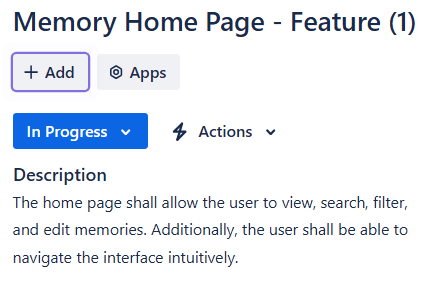
\includegraphics{snapshot1img1.png}\newline
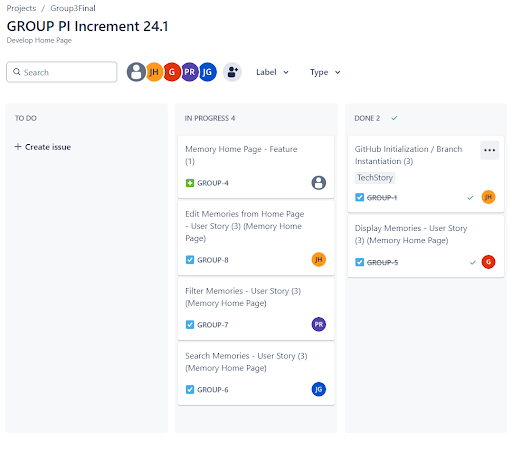
\includegraphics{snapshot1img2.png}
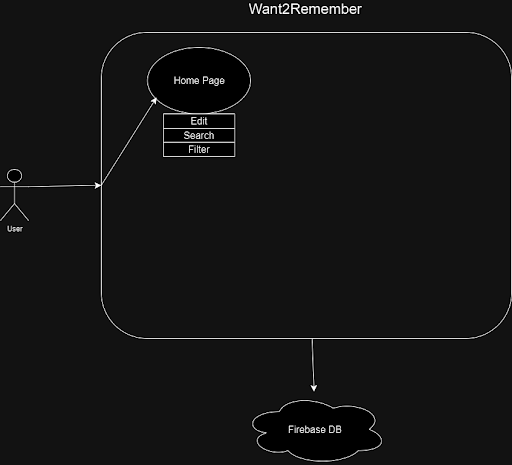
\includegraphics{snapshot1img3.png}
\textbf{Description:}The outer boundary represents the scope of the Want2Remember Product. Within shows different features as bubbles and their associated functionality as a table below. Outside of the boundary are external functionalities. The arrows represent the data flow of the product.


\subsection{Snapshot 2}
\textbf{Objective:} To create a page that will allow users to create memories that can later be accessed from the DB.\newline Dependencies Added :
\begin{itemize}
    \item
     TestRail
\end{itemize}
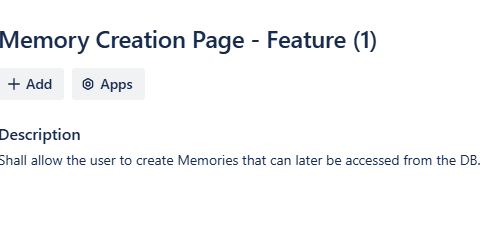
\includegraphics{snapshot2img1.png}
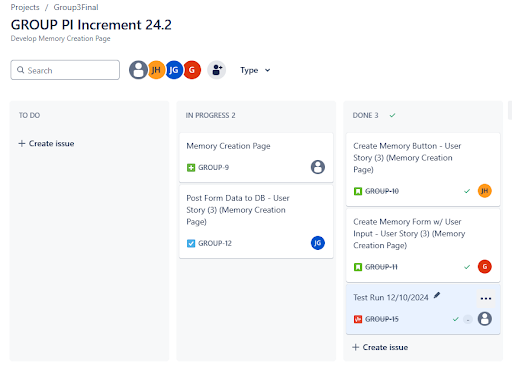
\includegraphics{snapshot2img2.png}
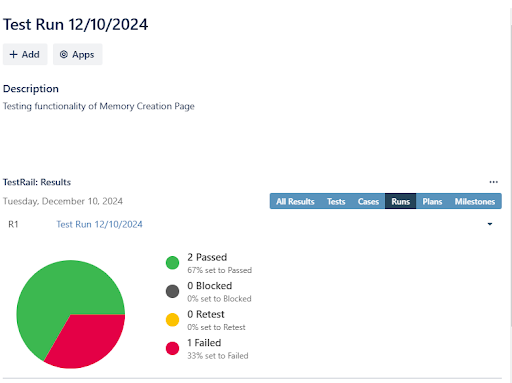
\includegraphics{snapshot2img3.png}
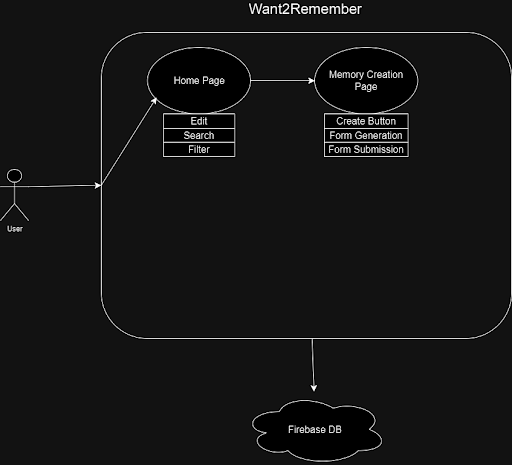
\includegraphics{snapshot2img4.png}

\subsection{Snapshot 3}
\textbf{Objective:} Complete the More Detail Page. \newline
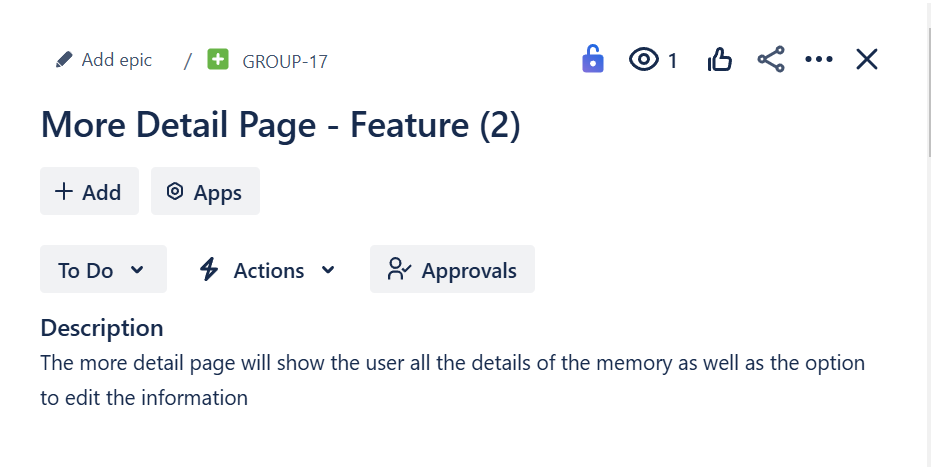
\includegraphics{snapshot3img1.png}
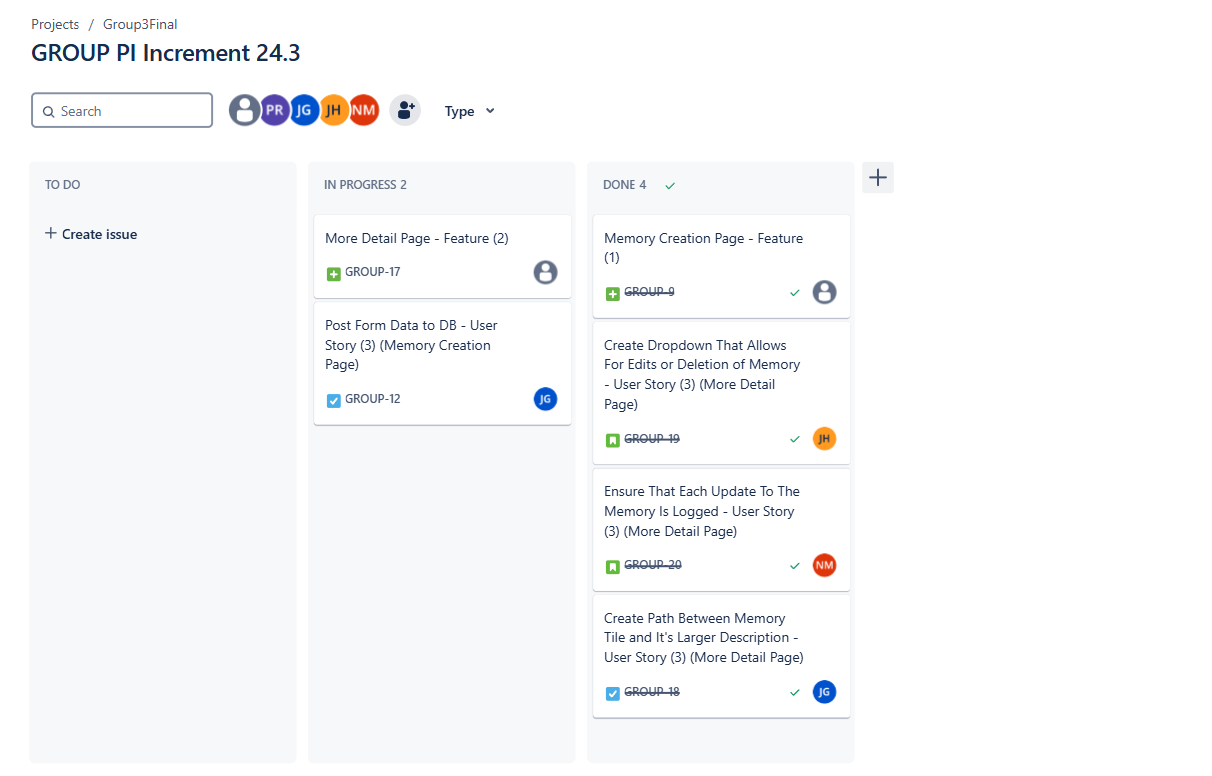
\includegraphics{snapshot3img2.png}
\includegraphics{snapshot3img3.png}

\subsection{Snapshot 4}
\textbf{Objective:} Memory Contact Page\newline
\includegraphics{snapshot4img1.png}\newline
\includegraphics{snapshot4img2.png}
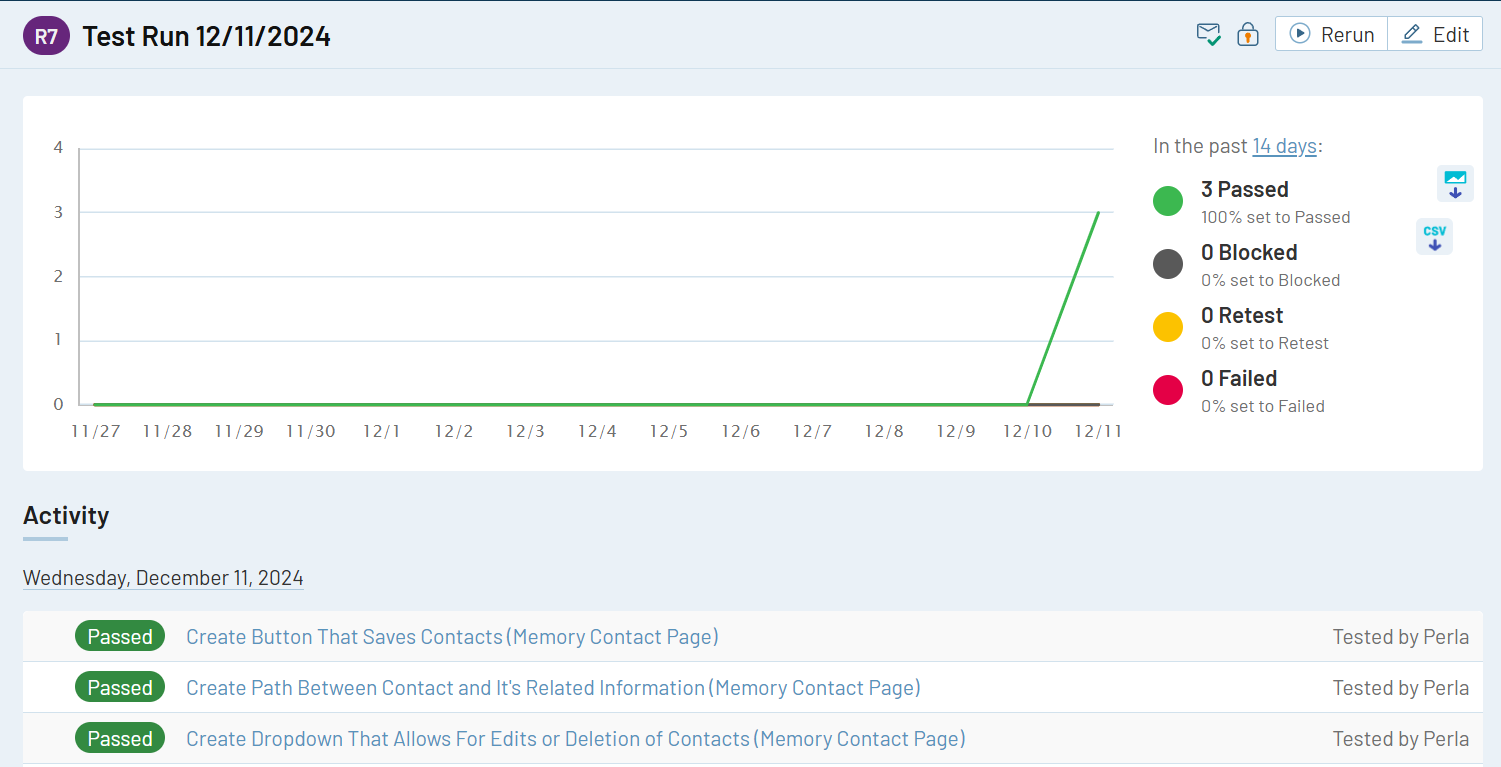
\includegraphics{snapshot4img3.png}



\end{document}

